\usetikzlibrary{arrows.meta, positioning, shapes.geometric}

\begin{figure}[ht]
\centering
\scalebox{0.5}{%
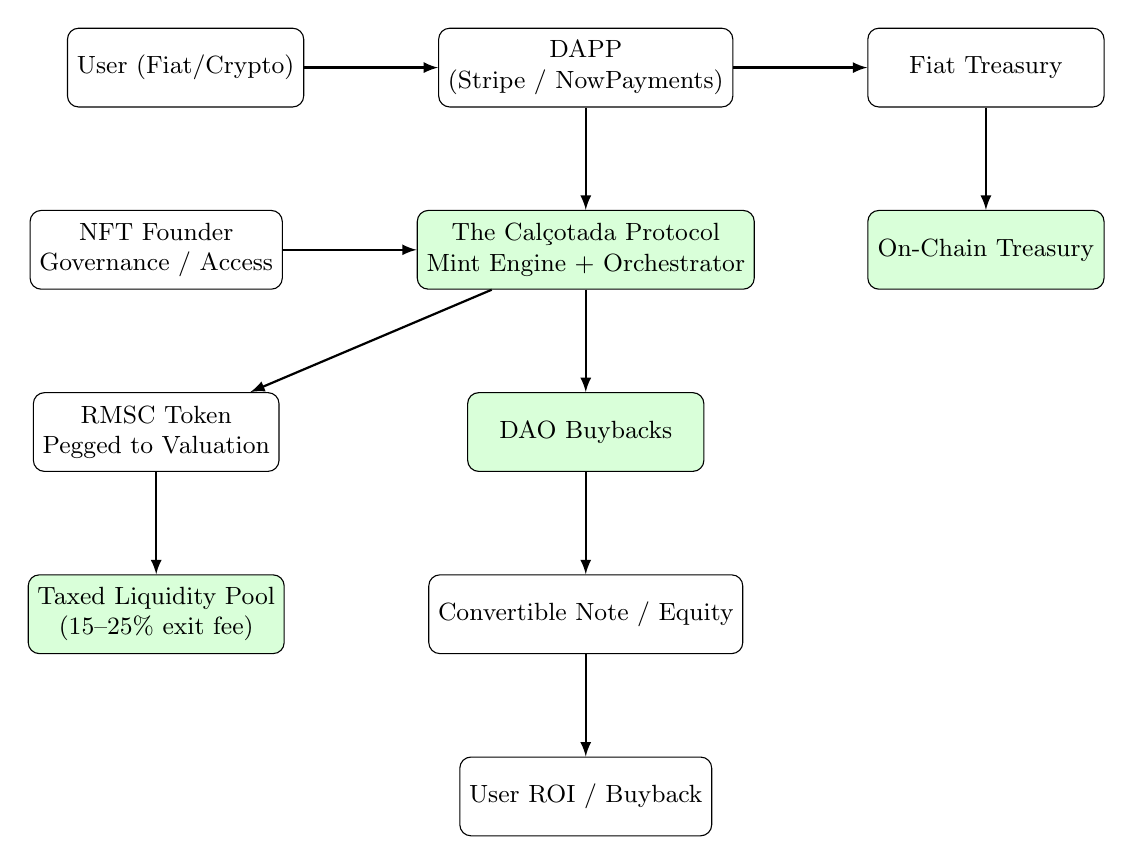
\begin{tikzpicture}[node distance=1.3cm and 1.7cm, every node/.style={font=\small}]

% Styles
\tikzstyle{box} = [draw, rounded corners, align=center, minimum width=3cm, minimum height=1cm, fill=white]
\tikzstyle{greenbox} = [box, fill=green!15]
\tikzstyle{arrow} = [->, thick, >=latex]

% Nodes
\node[box] (user) {User (Fiat/Crypto)};
\node[box, right=of user] (dapp) {DAPP\\(Stripe / NowPayments)};
\node[box, right=of dapp] (fiat) {Fiat Treasury};
\node[greenbox, below=of fiat] (onchain) {On-Chain Treasury};

\node[greenbox, below=of dapp] (protocol) {The Calçotada Protocol\\Mint Engine + Orchestrator};

\node[box, left=of protocol] (nft) {NFT Founder\\Governance / Access};
\node[box, below=of nft] (rmsc) {RMSC Token\\Pegged to Valuation};

\node[greenbox, below=of protocol] (dao) {DAO Buybacks};
\node[box, below=of dao] (equity) {Convertible Note / Equity};
\node[box, below=of equity] (payback) {User ROI / Buyback};

\node[greenbox, below=of rmsc] (tlp) {Taxed Liquidity Pool\\(15–25\% exit fee)};

% Arrows
\draw[arrow] (user) -- (dapp);
\draw[arrow] (dapp) -- (fiat);
\draw[arrow] (fiat) -- (onchain);
\draw[arrow] (dapp) -- (protocol);

\draw[arrow] (nft) -- (protocol);
\draw[arrow] (protocol) -- (rmsc);
\draw[arrow] (protocol) -- (dao);
\draw[arrow] (dao) -- (equity);
\draw[arrow] (equity) -- (payback);
\draw[arrow] (rmsc) -- (tlp);

\end{tikzpicture}%
}%
\caption{Simplified architecture of the Calçotada Protocol: dual-token issuance and treasury-integrated valuation peg.}
\end{figure}
